\section{Answers to Assignment Questions}

\noindent \textbf{Q1. After DROPping echo-reply packets on OUTPUT chain, what 
was the observed effect? Use Figure~\ref{fig:icmpexample} to illustrate the 
path of the packets. Mark the path with arrows and use an X to mark the point 
where the packets are DROPped.}

The ping requests got sent but no responses were received.
\\

\noindent \textbf{Q2. After DROPing echo-request packets on INPUT chain, what
was the observed effect? How is this reaction different from the reaction
achieved in Q1? Use Figure~\ref{fig:icmpexample} to illustrate the path of 
the packets. Mark the path with arrows and use an X to mark the point where the
packets are DROPped.}

The same thing happend here, the ping requests got sent without any problems but 
no answers were received. The difference in this case from the previous is that
when dropping the packets on the input the packet never reaches the 
icmp server and thereby needs less processing than in the case were it is dropped
on the output. This could be seen by the fact that when dropping on the input it 
is the request that is dropped while as when dropping on the output it is the 
generated response that is dropped.
\\

\begin{figure}[!ht]
    \begin{center}
        \subfigure[Use this Figure to explain Q1]{
           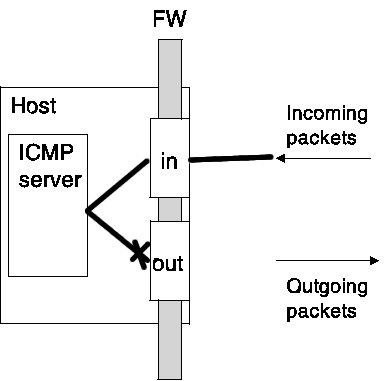
\includegraphics[scale=0.5]{figures/icmpexample-out}
           \label{fig:icmpexampleQ1}
        }
        \hspace{1in}
        \subfigure[Use this Figure to explain Q2]{
           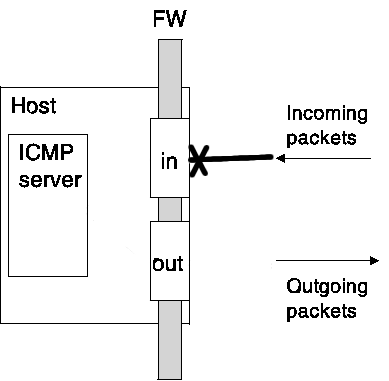
\includegraphics[scale=0.5]{figures/icmpexample-in}
           \label{fig:icmpexampleQ2}
        }
    \end{center}
    \caption{Figure to help you illustrate your thoughts regarding the packet 
        flow in questions Q1 and Q2.}
    \label{fig:icmpexample}
\end{figure}


\noindent \textbf{Q3. For each entry in the log, several information items are
displayed. Some entries can be useful for creating new rules. Explain the 
items {\texttt IN}, {\texttt OUT}, {\texttt SRC}, {\texttt DST} and {\texttt PROTO}
mean and why these might be useful.}
 
Not applicable. The logging did not work for anyone during the lab. File permissions?
\\

\noindent \textbf{Q4. At this stage, with default policy set to DROP for all 
chains, would you consider the system secure? Would you consider it useful?}

The system is most certainly secure but not usefull. If no traffic att all will
be let through the only security holes would be if there is any implementation 
bugs in the firwall. Other attacks like DoS will allso work. 
\\

\noindent \textbf{Q5. Assume instead that you used default policy ACCEPT, 
would you consider the system secure now? Would you consider it useful?}

With a policy of ACCEPT and no other rules everything will work without interference
from the firewall. This would be the same as turning the firewall off. If you add
the appropriate rules the system could be made just as secure as with policy DROP but
this aproach is much more prone to human error.
\\

\noindent \textbf{Q6. You just added some protection against flooding by 
limiting the number of packets the firewall will let through to 1 per second. 
Give two examples on how you can tell that you are protected!}

By sending a ping storm from another host and se that our host only responds to 1 per 
second. We can also use wireshark on the host an see that the host only handles 1 
ping per second.
